% !TeX program = pdflatex
\documentclass[border=6pt]{standalone}
\usepackage{tikz}
\usetikzlibrary{arrows.meta, positioning, calc, fit, backgrounds}

\definecolor{MediumRed}{rgb}{0.925, 0.345, 0.345}
\definecolor{MediumGreen}{rgb}{0.37, 0.7, 0.66}
\definecolor{MediumBlue}{rgb}{0.015, 0.315, 0.45}
\definecolor{DarkBlue}{rgb}{0.05, 0.15, 0.35}

% dibuja una rejilla 3 articulaciones (filas) x 3 fotogramas (columnas)
\newcommand{\grid}[1]{%
  \foreach \t in {0,1,2}
    \foreach \n in {0,1,2}
      \node[circle, fill=MediumBlue!35, minimum size=5pt, inner sep=0pt] (#1-\n-\t) at (\t*0.95,-\n*0.8) {};
}

\begin{document}
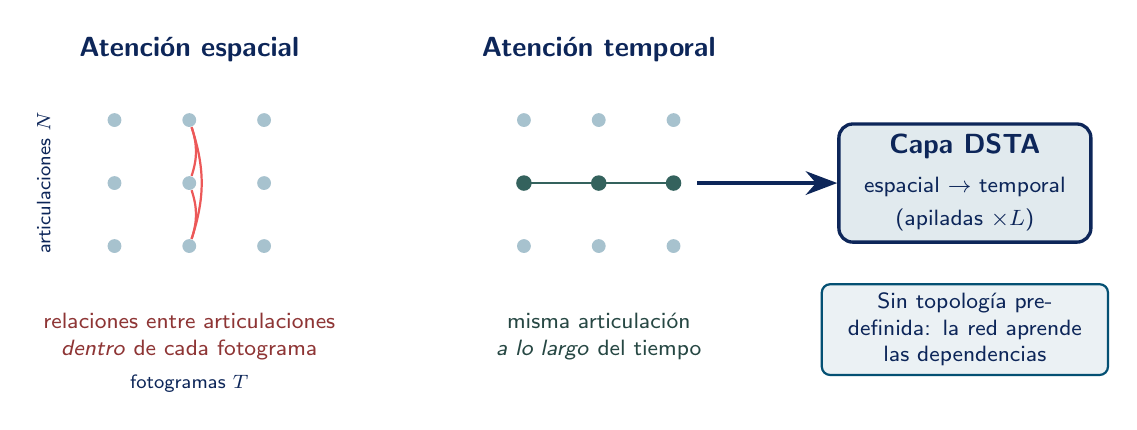
\begin{tikzpicture}[font=\sffamily]

% ================= PANEL ESPACIAL =================
\begin{scope}[shift={(0,0)}]
    \grid{S}
    % conexiones dentro de un mismo fotograma (columna t=1)
    \foreach \a/\b in {0/1,1/2,0/2}
        \draw[MediumRed, thick, bend left=18] (S-\a-1) to (S-\b-1);
    \node[font=\sffamily\bfseries, text=DarkBlue, align=center] at (0.95,0.9)
        {\textbf{Atención espacial}};
    \node[font=\sffamily\footnotesize, text=MediumRed!60!black, align=center] at (0.95,-2.75)
        {relaciones entre articulaciones\\ \emph{dentro} de cada fotograma};
\end{scope}

% ================= PANEL TEMPORAL =================
\begin{scope}[shift={(5.2,0)}]
    \grid{T}
    % conexiones de una misma articulacion a lo largo del tiempo (fila n=1)
    \draw[MediumGreen!55!black, thick] (T-1-0) -- (T-1-1) -- (T-1-2);
    \foreach \t in {0,1,2} \fill[MediumGreen!55!black] (T-1-\t) circle (2.8pt);
    \node[font=\sffamily\bfseries, text=DarkBlue, align=center] at (0.95,0.9)
        {\textbf{Atención temporal}};
    \node[font=\sffamily\footnotesize, text=MediumGreen!40!black, align=center] at (0.95,-2.75)
        {misma articulación\\ \emph{a lo largo} del tiempo};
\end{scope}

% ejes comunes
\node[font=\sffamily\scriptsize, text=DarkBlue, rotate=90] at (-0.9,-0.8) {articulaciones $N$};
\node[font=\sffamily\scriptsize, text=DarkBlue] at (0.95,-3.35) {fotogramas $T$};

% ================= SALIDA: capa DSTA =================
\node[draw=DarkBlue, very thick, rounded corners=5pt, fill=MediumBlue!12,
      text=DarkBlue, align=center, minimum width=3.2cm, minimum height=1.5cm]
      at (10.8,-0.8) (layer)
    {\textbf{Capa DSTA}\\[2pt]\footnotesize espacial $\rightarrow$ temporal\\\footnotesize (apiladas $\times L$)};
\draw[-{Stealth[length=4mm]}, line width=1.4pt, DarkBlue] (7.4,-0.8) -- (layer.west);

% nota clave
\node[draw=MediumBlue, thick, rounded corners=3pt, fill=MediumBlue!8,
      text=DarkBlue, font=\sffamily\footnotesize, align=center, text width=3.4cm,
      below=0.5cm of layer]
    {Sin topología predefinida: la red aprende las dependencias};

\end{tikzpicture}
\end{document}
